\documentclass[a4paper,11pt,notitlepage]{article}

\usepackage[T1]{fontenc}
\usepackage[utf8]{inputenc}
\usepackage[english, russian]{babel}
\usepackage{graphicx}
\graphicspath{ {./images/} }

\newcommand{\ans}{\textbf{Ответ: }}

\title{Теория игр, дз 1. Дорешивание.}
\author{Катя Гольцова}
\date{October 2018}

\begin{document}

\maketitle

\section{Теоретические задачи}
\subsection{Доминируемая стратегия}

Полностью решена при прошлой сдаче.

\subsection{Порядок удаления доминируемых стратегий}
\subsubsection{Строго доминируемые стратегии}

Докажем, что порядок удаления строго доминируемых стратегий не влияет на множество оставшихся стратегий. Это следует из двух фактов: (1) стратегии, которые становятся доминируемыми, одни и те же, и (2) любая доминируемая стратегия будет удалена.

\textit{(2): любая доминируемая стратегия будет удалена. Это верно, поскольку процесс удаления конечен (так как стратегий конечное число), и доминируемая стратегия никогда не перестанет быть доминируемой (пусть доминирующая её стратегия $s_2$ была удалена. Тогда $s_2$ была доминирована некоторой стратегией $s_3$, и, поскольку отношение доминируемости очевидным образом транзитивно, наша исходная стратегия доминируется стратегией $s_3$ и подлежит удалению).}

\textit{(1): пусть стратегия $s_1$ стала доминируемой. Это произошло после удаления 0 или больше профилей, содержащих её. Заметим, что эти профили были удалены, так как какие-то другие стратегии были удалены. Из (2) мы знаем, что эти стратегии будут удалены при любом порядке удаления, а значит, $s_1$ станет доминируемой при любом порядке удаления.}

\subsubsection{Слабо доминируемные стратегии}

Полностью решена при прошлой сдаче.

\subsection{Исключение строго доминируемых стратегий}

\textit{Пример:}

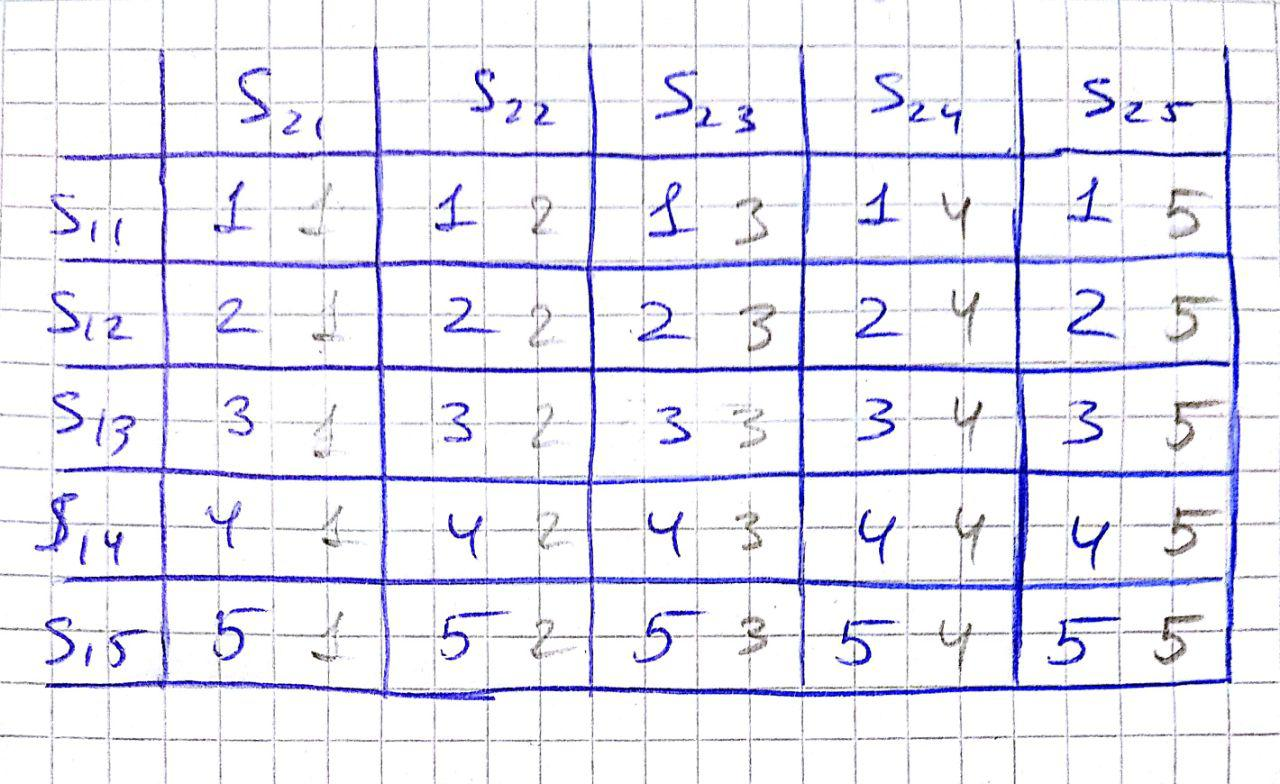
\includegraphics[scale=0.25]{example-1-6}

\textit{Порядок удаления: $s_{21} \rightarrow s_{22} \rightarrow s_{23} \rightarrow s_{24} \rightarrow s_{11} \rightarrow s_{12} \rightarrow s_{13} \rightarrow s_{14}$} 

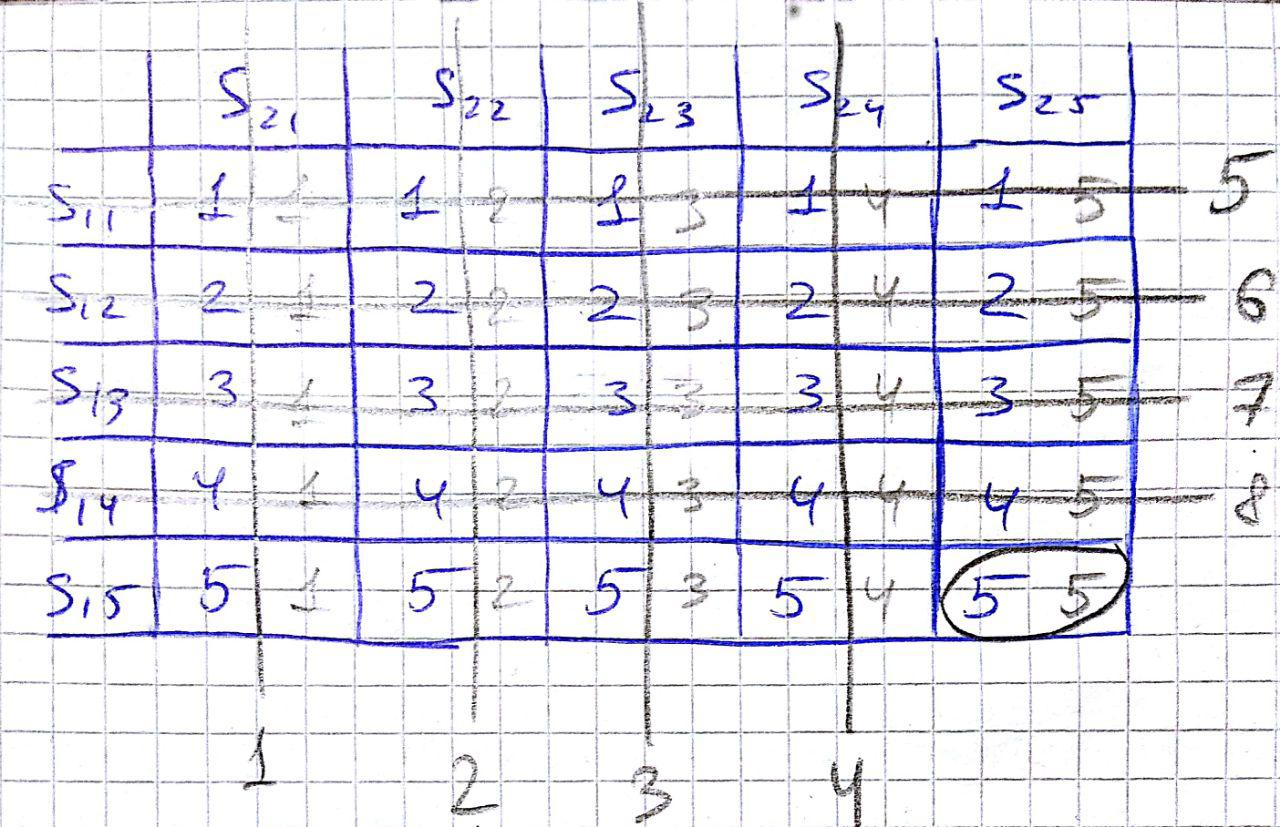
\includegraphics[scale=0.25]{example-1-7}

\subsection{Равновесия Нэша и Парето оптимальные исходы}

Полностью решена при прошлой сдаче.

\section{Аукцион второй цены}

Полностью решена при прошлой сдаче.

\section{Странный аукцион}
\subsection{Чистые равновесия Нэша}
Заметим, что $(a, b, c)$ -- равновесие, если ни один из игроков не может поменять свою ставку так, чтобы повысить полезность. Также заметим, что если $(a, b, c)$ -- профиль стратегий, то полезность хотя бы двух игроков из трёх при этом профиле равна 0. Таким образом, если какой-то игрок может сделать свою полезность ненулевой, то исход не является равновесием Нэша.

Пусть $(a, b, c)$ -- ставки. Поскольку мы рассматриваем набор ставок с точностью до перестановки, зафиксируем порядок $a \geq b \geq c$. Есть два принципиально разных типа исходов: 1) один из мужиков получает водку и 2) водка выливается. Рассмотрим, какие исходы могут быть равновесиями Нэша в каждом случае.

\begin{enumerate}
\item  Один из мужиков получает водку. Я утверждаю, что в таком случае его ставка может быть либо 9, либо 10. Действительно, раз другие мужики водки не получили, их ставки ниже, а полезность 0. Значит, будь ставка "успешного" мужика 8 или ниже, один из проигравших мог бы выбрать 9 и достичь полезности 1 -- следовательно, рассмотренный исход не являлся бы равновесием Нэша, т.к. один из игроков захотел бы отклониться от выбранной стратегии. Заметим также, что ставка 9 всё же возможна, т.к. хоть какой-то другой мужик и мог бы "перебить" ставку успешного, тем самым он не повысил бы свою полезность. \textit{Далее, заметим, что мужик, потративший 9 или 10 на водку, был бы не прочь потратить меньше. Значит, какой-то другой мужик должен потратить всего на 1 меньше (иначе наш выигравший мужик мог бы потратить меньше).}

\textit{Итого условия, которые выполняются в этом случае: $ a \in \{9,  10\}$, $ b = a - 1, c < b$ (знак строгий, так как водка не выливается). Значит, всего равновесий Нэша таких, что один из мужиков получает водку $7 + 8 = 15$.}

\item Водка выливается. Значит, 2 или 3 мужика сделали одну и ту же ставку. Т.е. возможны три случая (помним, что рассматриваем $a \geq b \geq c$):
	\begin{enumerate}
		\item $a = b = c$. Всего таких исходов 10.
		\item $a = b > c$. Заметим, что одна из ставок $a$ или $b$ могла бы быть повышена. В каких случаях это не улучшит полезность повысившего? -- Если повысить на самом деле нельзя ($a = b = 10$) или полезность повысившего остаётся нулевой (можно повысить только до 10, т.е. $a = b = 9$. Значит, всего таких случаев $\sum_{c = 1}^8 1 + \sum_{c=1}^9 1 = 8 + 9 = 17$.
		\item $a > b = c$. Опять же, повышение одной из равных ставок не должно повышать полезность. Значит, $a \in \{9, 10 \}$, и таких случаев тоже $17$.
	\end{enumerate}
	
Итого случаев из этого пункта (равновесия Нэша такие, что водка выливается) $10 + 17 + 17 = 44$.
\end{enumerate}

\ans в этой игре \textit{59} различных чистых равновесий Нэша.

\subsection{Равновесия Нэша: товар уничтожается}

\ans по рассуждениям из пункта 2 предыдущей секции, таких равновесий 44.

\subsection{Равновесия Нэша: чей-то выигрыш положителен}

\textit{Это такие исходы, при которых мужик получает водку, поставив меньше 10. По рассуждениям из пункта 1, таких 7.}

\section{Чистые и смешанные равновесия}

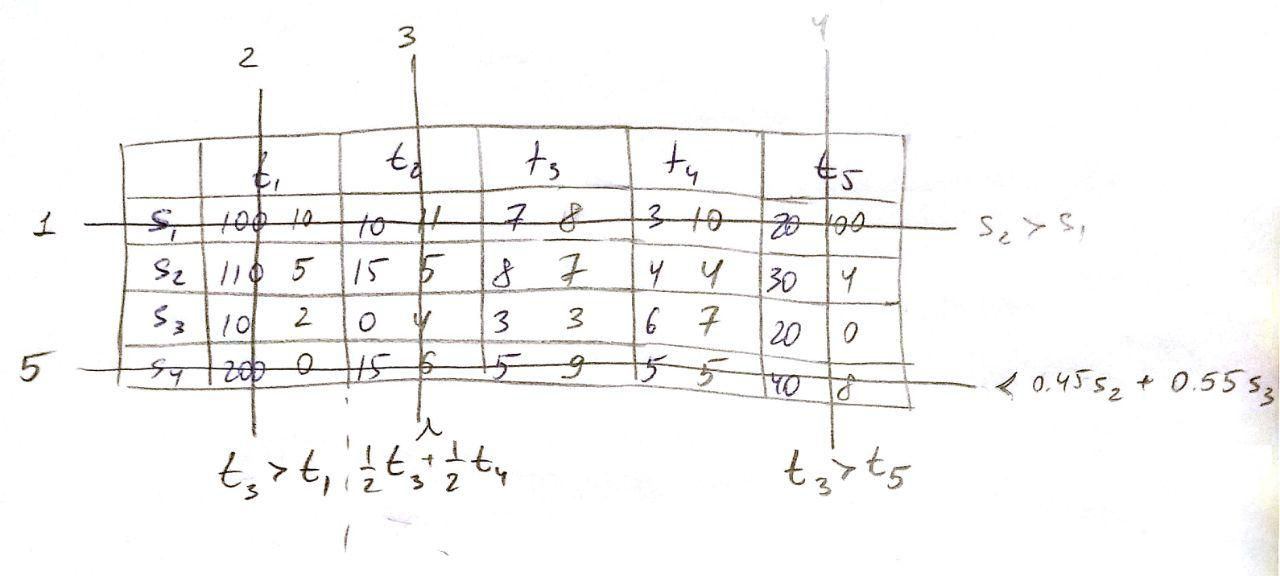
\includegraphics[scale=0.5]{photo-1}

$s_2 \succ s_1$.

После этого, $t_3 \succ t_1$.

После этого, $\frac{1}{2}t_3 + \frac{1}{2}t_4 \succ t_2$, а также $t_3 \succ t_5$.

Затем, $0.45 s_2 + 0.55 s_3 \succ s_4$.

Таким образом, чистые равновесия Нэша -- (8, 7) и (6, 7).

\textit{Рассмотрим смешанные равновесия Нэша. По тем же соображениям, что и в чистом случае, нет смысла рассматривать доминируемые стратегии -- следовательно, рассмотрим смеси стратегий $s_2$ и $s_3$ для первого игрока, $t_3$ и $t_4$ для второго игрока. Рассмотрим $\sigma_1 = p s_2 + (1-p) s_3$, $\sigma_2 = q t_3 + (1-q) t_4$. Тогда ожидаемые выигрыши: , }

\begin{itemize}
\item \textit{для 1-го игрока 
$$E_\sigma (u_1(s)) = 8pq + 4p(1-q) + 3(1-p)q + 6(1-p)(1-q) = p(7q - 2) + (6-3q)$$
Из условия "равновесности": если $q < \frac{2}{7}$, то $p = 0$, если $q = \frac{2}{7}$, то $p$ любое, если $q > \frac{2}{7}$, то $p = 1$.}
\item \textit{для 2-го игрока 
$$E_\sigma (u_2(s)) = 7pq + 4p(1-q) + 3(1-p)q + 7(1-p)(1-q) = q(7p - 4) + (7-3p)$$ 
Из условия "равновесности": если $p < \frac{4}{7}$, то $q = 0$, если $p = \frac{4}{7}$, то $q$ любое, если $p > \frac{4}{7}$, то $q = 1$.}
\end{itemize}

\textit{Решая эту систему, получаем смешанные равновесия Нэша при $p = 0, q = 0$, $p = 1, q = 1$ и $p = \frac{4}{7}, q = \frac{2}{7}$, то есть $\sigma = (s_2, t_3)$, $\sigma = (s_3, t_4)$ и $\sigma = (\frac{4}{7} s_2 + \frac{3}{7} s_3, \frac{2}{7} t_3 + \frac{5}{7} t_4)$ будут смешанными равновесиями Нэша.}

\end{document}
